\documentclass[12pt,a4paper,]{book}
\def\ifdoblecara{} %% set to true
\def\ifprincipal{} %% set to true
\let\ifprincipal\undefined %% set to false
\def\ifcitapandoc{} %% set to true
\let\ifcitapandoc\undefined %% set to false
\usepackage{lmodern}
% sin fontmathfamily
\usepackage{amssymb,amsmath}
\usepackage{ifxetex,ifluatex}
%\usepackage{fixltx2e} % provides \textsubscript %PLLC
\ifnum 0\ifxetex 1\fi\ifluatex 1\fi=0 % if pdftex
  \usepackage[T1]{fontenc}
  \usepackage[utf8]{inputenc}
\else % if luatex or xelatex
  \ifxetex
    \usepackage{mathspec}
  \else
    \usepackage{fontspec}
  \fi
  \defaultfontfeatures{Ligatures=TeX,Scale=MatchLowercase}
\fi
% use upquote if available, for straight quotes in verbatim environments
\IfFileExists{upquote.sty}{\usepackage{upquote}}{}
% use microtype if available
\IfFileExists{microtype.sty}{%
\usepackage{microtype}
\UseMicrotypeSet[protrusion]{basicmath} % disable protrusion for tt fonts
}{}
\usepackage[margin = 2.5cm]{geometry}
\usepackage{hyperref}
\hypersetup{unicode=true,
            pdfauthor={Nombre Completo Autor},
              pdfborder={0 0 0},
              breaklinks=true}
\urlstyle{same}  % don't use monospace font for urls
%
\usepackage[usenames,dvipsnames]{xcolor}  %new PLLC
\usepackage{color}
\usepackage{fancyvrb}
\newcommand{\VerbBar}{|}
\newcommand{\VERB}{\Verb[commandchars=\\\{\}]}
\DefineVerbatimEnvironment{Highlighting}{Verbatim}{commandchars=\\\{\}}
% Add ',fontsize=\small' for more characters per line
\usepackage{framed}
\definecolor{shadecolor}{RGB}{248,248,248}
\newenvironment{Shaded}{\begin{snugshade}}{\end{snugshade}}
\newcommand{\AlertTok}[1]{\textcolor[rgb]{0.94,0.16,0.16}{#1}}
\newcommand{\AnnotationTok}[1]{\textcolor[rgb]{0.56,0.35,0.01}{\textbf{\textit{#1}}}}
\newcommand{\AttributeTok}[1]{\textcolor[rgb]{0.13,0.29,0.53}{#1}}
\newcommand{\BaseNTok}[1]{\textcolor[rgb]{0.00,0.00,0.81}{#1}}
\newcommand{\BuiltInTok}[1]{#1}
\newcommand{\CharTok}[1]{\textcolor[rgb]{0.31,0.60,0.02}{#1}}
\newcommand{\CommentTok}[1]{\textcolor[rgb]{0.56,0.35,0.01}{\textit{#1}}}
\newcommand{\CommentVarTok}[1]{\textcolor[rgb]{0.56,0.35,0.01}{\textbf{\textit{#1}}}}
\newcommand{\ConstantTok}[1]{\textcolor[rgb]{0.56,0.35,0.01}{#1}}
\newcommand{\ControlFlowTok}[1]{\textcolor[rgb]{0.13,0.29,0.53}{\textbf{#1}}}
\newcommand{\DataTypeTok}[1]{\textcolor[rgb]{0.13,0.29,0.53}{#1}}
\newcommand{\DecValTok}[1]{\textcolor[rgb]{0.00,0.00,0.81}{#1}}
\newcommand{\DocumentationTok}[1]{\textcolor[rgb]{0.56,0.35,0.01}{\textbf{\textit{#1}}}}
\newcommand{\ErrorTok}[1]{\textcolor[rgb]{0.64,0.00,0.00}{\textbf{#1}}}
\newcommand{\ExtensionTok}[1]{#1}
\newcommand{\FloatTok}[1]{\textcolor[rgb]{0.00,0.00,0.81}{#1}}
\newcommand{\FunctionTok}[1]{\textcolor[rgb]{0.13,0.29,0.53}{\textbf{#1}}}
\newcommand{\ImportTok}[1]{#1}
\newcommand{\InformationTok}[1]{\textcolor[rgb]{0.56,0.35,0.01}{\textbf{\textit{#1}}}}
\newcommand{\KeywordTok}[1]{\textcolor[rgb]{0.13,0.29,0.53}{\textbf{#1}}}
\newcommand{\NormalTok}[1]{#1}
\newcommand{\OperatorTok}[1]{\textcolor[rgb]{0.81,0.36,0.00}{\textbf{#1}}}
\newcommand{\OtherTok}[1]{\textcolor[rgb]{0.56,0.35,0.01}{#1}}
\newcommand{\PreprocessorTok}[1]{\textcolor[rgb]{0.56,0.35,0.01}{\textit{#1}}}
\newcommand{\RegionMarkerTok}[1]{#1}
\newcommand{\SpecialCharTok}[1]{\textcolor[rgb]{0.81,0.36,0.00}{\textbf{#1}}}
\newcommand{\SpecialStringTok}[1]{\textcolor[rgb]{0.31,0.60,0.02}{#1}}
\newcommand{\StringTok}[1]{\textcolor[rgb]{0.31,0.60,0.02}{#1}}
\newcommand{\VariableTok}[1]{\textcolor[rgb]{0.00,0.00,0.00}{#1}}
\newcommand{\VerbatimStringTok}[1]{\textcolor[rgb]{0.31,0.60,0.02}{#1}}
\newcommand{\WarningTok}[1]{\textcolor[rgb]{0.56,0.35,0.01}{\textbf{\textit{#1}}}}

% PLLC modifica-ini
% PLLC modifica-fin

\IfFileExists{parskip.sty}{%
\usepackage{parskip}
}{% else
\setlength{\parindent}{0pt}
\setlength{\parskip}{6pt plus 2pt minus 1pt}
}
\setlength{\emergencystretch}{3em}  % prevent overfull lines
\providecommand{\tightlist}{%
  \setlength{\itemsep}{0pt}\setlength{\parskip}{0pt}}
\setcounter{secnumdepth}{5}
% Redefines (sub)paragraphs to behave more like sections
\ifx\paragraph\undefined\else
\let\oldparagraph\paragraph
\renewcommand{\paragraph}[1]{\oldparagraph{#1}\mbox{}}
\fi
\ifx\subparagraph\undefined\else
\let\oldsubparagraph\subparagraph
\renewcommand{\subparagraph}[1]{\oldsubparagraph{#1}\mbox{}}
\fi

%%% Use protect on footnotes to avoid problems with footnotes in titles
\let\rmarkdownfootnote\footnote%
\def\footnote{\protect\rmarkdownfootnote}


  \title{}
    \author{Nombre Completo Autor}
      \date{18/11/2021}


%%%%%%% inicio: latex_preambulo.tex PLLC


%% UTILIZA CODIFICACIÓN UTF-8
%% MODIFICARLO CONVENIENTEMENTE PARA USARLO CON OTRAS CODIFICACIONES


%\usepackage[spanish,es-nodecimaldot,es-noshorthands]{babel}
\usepackage[spanish,es-nodecimaldot,es-noshorthands,es-tabla]{babel}
% Ver: es-tabla (en: https://osl.ugr.es/CTAN/macros/latex/contrib/babel-contrib/spanish/spanish.pdf)
% es-tabla (en: https://tex.stackexchange.com/questions/80443/change-the-word-table-in-table-captions)
\usepackage[spanish, plain, datebegin,sortcompress,nocomment,
noabstract]{flexbib}
 
\usepackage{float}
\usepackage{placeins}
\usepackage{fancyhdr}
% Solucion: ! LaTeX Error: Command \counterwithout already defined.
% https://tex.stackexchange.com/questions/425600/latex-error-command-counterwithout-already-defined
\let\counterwithout\relax
\let\counterwithin\relax
\usepackage{chngcntr}
%\usepackage{microtype}  %antes en template PLLC
\usepackage[utf8]{inputenc}
\usepackage[T1]{fontenc} % Usa codificación 8-bit que tiene 256 glyphs

%\usepackage[dvipsnames]{xcolor}
%\usepackage[usenames,dvipsnames]{xcolor}  %new
\usepackage{pdfpages}
%\usepackage{natbib}




% Para portada: latex_paginatitulo_mod_ST02.tex (inicio)
\usepackage{tikz}
\usepackage{epigraph}
\input{portadas/latex_paginatitulo_mod_ST02_add.sty}
% Para portada: latex_paginatitulo_mod_ST02.tex (fin)

% Para portada: latex_paginatitulo_mod_OV01.tex (inicio)
\usepackage{cpimod}
% Para portada: latex_paginatitulo_mod_OV01.tex (fin)

% Para portada: latex_paginatitulo_mod_OV03.tex (inicio)
\usepackage{KTHEEtitlepage}
% Para portada: latex_paginatitulo_mod_OV03.tex (fin)

\renewcommand{\contentsname}{Índice}
\renewcommand{\listfigurename}{Índice de figuras}
\renewcommand{\listtablename}{Índice de tablas}
\newcommand{\bcols}{}
\newcommand{\ecols}{}
\newcommand{\bcol}[1]{\begin{minipage}{#1\linewidth}}
\newcommand{\ecol}{\end{minipage}}
\newcommand{\balertblock}[1]{\begin{alertblock}{#1}}
\newcommand{\ealertblock}{\end{alertblock}}
\newcommand{\bitemize}{\begin{itemize}}
\newcommand{\eitemize}{\end{itemize}}
\newcommand{\benumerate}{\begin{enumerate}}
\newcommand{\eenumerate}{\end{enumerate}}
\newcommand{\saltopagina}{\newpage}
\newcommand{\bcenter}{\begin{center}}
\newcommand{\ecenter}{\end{center}}
\newcommand{\beproof}{\begin{proof}} %new
\newcommand{\eeproof}{\end{proof}} %new
%De: https://texblog.org/2007/11/07/headerfooter-in-latex-with-fancyhdr/
% \fancyhead
% E: Even page
% O: Odd page
% L: Left field
% C: Center field
% R: Right field
% H: Header
% F: Footer
%\fancyhead[CO,CE]{Resultados}

%OPCION 1
% \fancyhead[LE,RO]{\slshape \rightmark}
% \fancyhead[LO,RE]{\slshape \leftmark}
% \fancyfoot[C]{\thepage}
% \renewcommand{\headrulewidth}{0.4pt}
% \renewcommand{\footrulewidth}{0pt}

%OPCION 2
% \fancyhead[LE,RO]{\slshape \rightmark}
% \fancyfoot[LO,RE]{\slshape \leftmark}
% \fancyfoot[LE,RO]{\thepage}
% \renewcommand{\headrulewidth}{0.4pt}
% \renewcommand{\footrulewidth}{0.4pt}
%%%%%%%%%%
\usepackage{calc,amsfonts}
% Elimina la cabecera de páginas impares vacías al finalizar los capítulos
\usepackage{emptypage}
\makeatletter

%\definecolor{ocre}{RGB}{25,25,243} % Define el color azul (naranja) usado para resaltar algunas salidas
\definecolor{ocre}{RGB}{0,0,0} % Define el color a negro (aparece en los teoremas

%\usepackage{calc} 


%era if(csl-refs) con dolares
% metodobib: true


\usepackage{lipsum}

%\usepackage{tikz} % Requerido para dibujar formas personalizadas

%\usepackage{amsmath,amsthm,amssymb,amsfonts}
\usepackage{amsthm}


% Boxed/framed environments
\newtheoremstyle{ocrenumbox}% % Theorem style name
{0pt}% Space above
{0pt}% Space below
{\normalfont}% % Body font
{}% Indent amount
{\small\bf\sffamily\color{ocre}}% % Theorem head font
{\;}% Punctuation after theorem head
{0.25em}% Space after theorem head
{\small\sffamily\color{ocre}\thmname{#1}\nobreakspace\thmnumber{\@ifnotempty{#1}{}\@upn{#2}}% Theorem text (e.g. Theorem 2.1)
\thmnote{\nobreakspace\the\thm@notefont\sffamily\bfseries\color{black}---\nobreakspace#3.}} % Optional theorem note
\renewcommand{\qedsymbol}{$\blacksquare$}% Optional qed square

\newtheoremstyle{blacknumex}% Theorem style name
{5pt}% Space above
{5pt}% Space below
{\normalfont}% Body font
{} % Indent amount
{\small\bf\sffamily}% Theorem head font
{\;}% Punctuation after theorem head
{0.25em}% Space after theorem head
{\small\sffamily{\tiny\ensuremath{\blacksquare}}\nobreakspace\thmname{#1}\nobreakspace\thmnumber{\@ifnotempty{#1}{}\@upn{#2}}% Theorem text (e.g. Theorem 2.1)
\thmnote{\nobreakspace\the\thm@notefont\sffamily\bfseries---\nobreakspace#3.}}% Optional theorem note

\newtheoremstyle{blacknumbox} % Theorem style name
{0pt}% Space above
{0pt}% Space below
{\normalfont}% Body font
{}% Indent amount
{\small\bf\sffamily}% Theorem head font
{\;}% Punctuation after theorem head
{0.25em}% Space after theorem head
{\small\sffamily\thmname{#1}\nobreakspace\thmnumber{\@ifnotempty{#1}{}\@upn{#2}}% Theorem text (e.g. Theorem 2.1)
\thmnote{\nobreakspace\the\thm@notefont\sffamily\bfseries---\nobreakspace#3.}}% Optional theorem note

% Non-boxed/non-framed environments
\newtheoremstyle{ocrenum}% % Theorem style name
{5pt}% Space above
{5pt}% Space below
{\normalfont}% % Body font
{}% Indent amount
{\small\bf\sffamily\color{ocre}}% % Theorem head font
{\;}% Punctuation after theorem head
{0.25em}% Space after theorem head
{\small\sffamily\color{ocre}\thmname{#1}\nobreakspace\thmnumber{\@ifnotempty{#1}{}\@upn{#2}}% Theorem text (e.g. Theorem 2.1)
\thmnote{\nobreakspace\the\thm@notefont\sffamily\bfseries\color{black}---\nobreakspace#3.}} % Optional theorem note
\renewcommand{\qedsymbol}{$\blacksquare$}% Optional qed square
\makeatother



% Define el estilo texto theorem para cada tipo definido anteriormente
\newcounter{dummy} 
\numberwithin{dummy}{section}
\theoremstyle{ocrenumbox}
\newtheorem{theoremeT}[dummy]{Teorema}  % (Pedro: Theorem)
\newtheorem{problem}{Problema}[chapter]  % (Pedro: Problem)
\newtheorem{exerciseT}{Ejercicio}[chapter] % (Pedro: Exercise)
\theoremstyle{blacknumex}
\newtheorem{exampleT}{Ejemplo}[chapter] % (Pedro: Example)
\theoremstyle{blacknumbox}
\newtheorem{vocabulary}{Vocabulario}[chapter]  % (Pedro: Vocabulary)
\newtheorem{definitionT}{Definición}[section]  % (Pedro: Definition)
\newtheorem{corollaryT}[dummy]{Corolario}  % (Pedro: Corollary)
\theoremstyle{ocrenum}
\newtheorem{proposition}[dummy]{Proposición} % (Pedro: Proposition)


\usepackage[framemethod=default]{mdframed}



\newcommand{\intoo}[2]{\mathopen{]}#1\,;#2\mathclose{[}}
\newcommand{\ud}{\mathop{\mathrm{{}d}}\mathopen{}}
\newcommand{\intff}[2]{\mathopen{[}#1\,;#2\mathclose{]}}
\newtheorem{notation}{Notation}[chapter]


\mdfdefinestyle{exampledefault}{%
rightline=true,innerleftmargin=10,innerrightmargin=10,
frametitlerule=true,frametitlerulecolor=green,
frametitlebackgroundcolor=yellow,
frametitlerulewidth=2pt}


% Theorem box
\newmdenv[skipabove=7pt,
skipbelow=7pt,
backgroundcolor=black!5,
linecolor=ocre,
innerleftmargin=5pt,
innerrightmargin=5pt,
innertopmargin=10pt,%5pt
leftmargin=0cm,
rightmargin=0cm,
innerbottommargin=5pt]{tBox}

% Exercise box	  
\newmdenv[skipabove=7pt,
skipbelow=7pt,
rightline=false,
leftline=true,
topline=false,
bottomline=false,
backgroundcolor=ocre!10,
linecolor=ocre,
innerleftmargin=5pt,
innerrightmargin=5pt,
innertopmargin=10pt,%5pt
innerbottommargin=5pt,
leftmargin=0cm,
rightmargin=0cm,
linewidth=4pt]{eBox}	

% Definition box
\newmdenv[skipabove=7pt,
skipbelow=7pt,
rightline=false,
leftline=true,
topline=false,
bottomline=false,
linecolor=ocre,
innerleftmargin=5pt,
innerrightmargin=5pt,
innertopmargin=10pt,%0pt
leftmargin=0cm,
rightmargin=0cm,
linewidth=4pt,
innerbottommargin=0pt]{dBox}	

% Corollary box
\newmdenv[skipabove=7pt,
skipbelow=7pt,
rightline=false,
leftline=true,
topline=false,
bottomline=false,
linecolor=gray,
backgroundcolor=black!5,
innerleftmargin=5pt,
innerrightmargin=5pt,
innertopmargin=10pt,%5pt
leftmargin=0cm,
rightmargin=0cm,
linewidth=4pt,
innerbottommargin=5pt]{cBox}

% Crea un entorno para cada tipo de theorem y le asigna un estilo 
% con ayuda de las cajas coloreadas anteriores
\newenvironment{theorem}{\begin{tBox}\begin{theoremeT}}{\end{theoremeT}\end{tBox}}
\newenvironment{exercise}{\begin{eBox}\begin{exerciseT}}{\hfill{\color{ocre}\tiny\ensuremath{\blacksquare}}\end{exerciseT}\end{eBox}}				  
\newenvironment{definition}{\begin{dBox}\begin{definitionT}}{\end{definitionT}\end{dBox}}	
\newenvironment{example}{\begin{exampleT}}{\hfill{\tiny\ensuremath{\blacksquare}}\end{exampleT}}		
\newenvironment{corollary}{\begin{cBox}\begin{corollaryT}}{\end{corollaryT}\end{cBox}}	

%	ENVIRONMENT remark
\newenvironment{remark}{\par\vspace{10pt}\small 
% Espacio blanco vertical sobre la nota y tamaño de fuente menor
\begin{list}{}{
\leftmargin=35pt % Indentación sobre la izquierda
\rightmargin=25pt}\item\ignorespaces % Indentación sobre la derecha
\makebox[-2.5pt]{\begin{tikzpicture}[overlay]
\node[draw=ocre!60,line width=1pt,circle,fill=ocre!25,font=\sffamily\bfseries,inner sep=2pt,outer sep=0pt] at (-15pt,0pt){\textcolor{ocre}{N}}; \end{tikzpicture}} % R naranja en un círculo (Pedro)
\advance\baselineskip -1pt}{\end{list}\vskip5pt} 
% Espaciado de línea más estrecho y espacio en blanco después del comentario


\newenvironment{solutionExe}{\par\vspace{10pt}\small 
\begin{list}{}{
\leftmargin=35pt 
\rightmargin=25pt}\item\ignorespaces 
\makebox[-2.5pt]{\begin{tikzpicture}[overlay]
\node[draw=ocre!60,line width=1pt,circle,fill=ocre!25,font=\sffamily\bfseries,inner sep=2pt,outer sep=0pt] at (-15pt,0pt){\textcolor{ocre}{S}}; \end{tikzpicture}} 
\advance\baselineskip -1pt}{\end{list}\vskip5pt} 

\newenvironment{solutionExa}{\par\vspace{10pt}\small 
\begin{list}{}{
\leftmargin=35pt 
\rightmargin=25pt}\item\ignorespaces 
\makebox[-2.5pt]{\begin{tikzpicture}[overlay]
\node[draw=ocre!60,line width=1pt,circle,fill=ocre!55,font=\sffamily\bfseries,inner sep=2pt,outer sep=0pt] at (-15pt,0pt){\textcolor{ocre}{S}}; \end{tikzpicture}} 
\advance\baselineskip -1pt}{\end{list}\vskip5pt} 

\usepackage{tcolorbox}

\usetikzlibrary{trees}

\theoremstyle{ocrenum}
\newtheorem{solutionT}[dummy]{Solución}  % (Pedro: Corollary)
\newenvironment{solution}{\begin{cBox}\begin{solutionT}}{\end{solutionT}\end{cBox}}	


\newcommand{\tcolorboxsolucion}[2]{%
\begin{tcolorbox}[colback=green!5!white,colframe=green!75!black,title=#1] 
 #2
 %\tcblower  % pone una línea discontinua
\end{tcolorbox}
}% final definición comando

\newtcbox{\mybox}[1][green]{on line,
arc=0pt,outer arc=0pt,colback=#1!10!white,colframe=#1!50!black, boxsep=0pt,left=1pt,right=1pt,top=2pt,bottom=2pt, boxrule=0pt,bottomrule=1pt,toprule=1pt}



\mdfdefinestyle{exampledefault}{%
rightline=true,innerleftmargin=10,innerrightmargin=10,
frametitlerule=true,frametitlerulecolor=green,
frametitlebackgroundcolor=yellow,
frametitlerulewidth=2pt}





\newcommand{\betheorem}{\begin{theorem}}
\newcommand{\eetheorem}{\end{theorem}}
\newcommand{\bedefinition}{\begin{definition}}
\newcommand{\eedefinition}{\end{definition}}

\newcommand{\beremark}{\begin{remark}}
\newcommand{\eeremark}{\end{remark}}
\newcommand{\beexercise}{\begin{exercise}}
\newcommand{\eeexercise}{\end{exercise}}
\newcommand{\beexample}{\begin{example}}
\newcommand{\eeexample}{\end{example}}
\newcommand{\becorollary}{\begin{corollary}}
\newcommand{\eecorollary}{\end{corollary}}


\newcommand{\besolutionExe}{\begin{solutionExe}}
\newcommand{\eesolutionExe}{\end{solutionExe}}
\newcommand{\besolutionExa}{\begin{solutionExa}}
\newcommand{\eesolutionExa}{\end{solutionExa}}


%%%%%%%%


% Caja Salida Markdown
\newmdenv[skipabove=7pt,
skipbelow=7pt,
rightline=false,
leftline=true,
topline=false,
bottomline=false,
backgroundcolor=GreenYellow!10,
linecolor=GreenYellow!80,
innerleftmargin=5pt,
innerrightmargin=5pt,
innertopmargin=10pt,%5pt
innerbottommargin=5pt,
leftmargin=0cm,
rightmargin=0cm,
linewidth=4pt]{mBox}	

%% RMarkdown
\newenvironment{markdownsal}{\begin{mBox}}{\end{mBox}}	

\newcommand{\bmarkdownsal}{\begin{markdownsal}}
\newcommand{\emarkdownsal}{\end{markdownsal}}


\usepackage{array}
\usepackage{multirow}
\usepackage{wrapfig}
\usepackage{colortbl}
\usepackage{pdflscape}
\usepackage{tabu}
\usepackage{threeparttable}
\usepackage{subfig} %new
%\usepackage{booktabs,dcolumn,rotating,thumbpdf,longtable}
\usepackage{dcolumn,rotating}  %new
\usepackage[graphicx]{realboxes} %new de: https://stackoverflow.com/questions/51633434/prevent-pagebreak-in-kableextra-landscape-table

%define el interlineado vertical
%\renewcommand{\baselinestretch}{1.5}

%define etiqueta para las Tablas o Cuadros
%\renewcommand\spanishtablename{Tabla}

%%\bibliographystyle{plain} %new no necesario


%%%%%%%%%%%% PARA USO CON biblatex
% \DefineBibliographyStrings{english}{%
%   backrefpage = {ver pag.\adddot},%
%   backrefpages = {ver pags.\adddot}%
% }

% \DefineBibliographyStrings{spanish}{%
%   backrefpage = {ver pag.\adddot},%
%   backrefpages = {ver pags.\adddot}%
% }
% 
% \DeclareFieldFormat{pagerefformat}{\mkbibparens{{\color{red}\mkbibemph{#1}}}}
% \renewbibmacro*{pageref}{%
%   \iflistundef{pageref}
%     {}
%     {\printtext[pagerefformat]{%
%        \ifnumgreater{\value{pageref}}{1}
%          {\bibstring{backrefpages}\ppspace}
%          {\bibstring{backrefpage}\ppspace}%
%        \printlist[pageref][-\value{listtotal}]{pageref}}}}
% 
%%% de kableExtra
\usepackage{booktabs}
\usepackage{longtable}
%\usepackage{array}
%\usepackage{multirow}
%\usepackage{wrapfig}
%\usepackage{float}
%\usepackage{colortbl}
%\usepackage{pdflscape}
%\usepackage{tabu}
%\usepackage{threeparttable}
\usepackage{threeparttablex}
\usepackage[normalem]{ulem}
\usepackage{makecell}
%\usepackage{xcolor}

%%%%%%% fin: latex_preambulo.tex PLLC


\begin{document}

\bibliographystyle{flexbib}



\raggedbottom

\ifdefined\ifprincipal
\else
\setlength{\parindent}{1em}
\pagestyle{fancy}
\setcounter{tocdepth}{4}
\tableofcontents

\fi

\ifdefined\ifdoblecara
\fancyhead{}{}
\fancyhead[LE,RO]{\scriptsize\rightmark}
\fancyfoot[LO,RE]{\scriptsize\slshape \leftmark}
\fancyfoot[C]{}
\fancyfoot[LE,RO]{\footnotesize\thepage}
\else
\fancyhead{}{}
\fancyhead[RO]{\scriptsize\rightmark}
\fancyfoot[LO]{\scriptsize\slshape \leftmark}
\fancyfoot[C]{}
\fancyfoot[RO]{\footnotesize\thepage}
\fi

\renewcommand{\headrulewidth}{0.4pt}
\renewcommand{\footrulewidth}{0.4pt}

\hypertarget{Seccion2}{%
\chapter{Tipos y formas de un juego. Equilibrio de
Nash}\label{Seccion2}}

\hypertarget{Seccion21}{%
\section{Tipos de juego}\label{Seccion21}}

\emph{Juegos según el número de jugadores}

Según el numero de jugadores nos encontramos con los juegos
bipersonales, de 2 personas como puede ser el ajedrez, o n-personales en
el que participan mas de 2 jugadores como en el poker.

\emph{Juegos cooperativos y no cooperativos}

\hypertarget{Seccion22}{%
\section{Formas de representacion de un juego}\label{Seccion22}}

\hypertarget{Seccion221}{%
\subsection{Forma normal o estratégica}\label{Seccion221}}

Comenzamos con la manera mas sencilla de representar un juego. En ella
asumimos que los jugadores toman sus decisiones a la vez sin conocer las
decisiones de los otros jugadores. Se asume como comentamos
anteriormente en la sección \(\ref{Seccion12}\) que los jugadores actúan
racionalmente y que siguen la estrategia (concepto que se definió
también al final del subapartado \(\ref{Seccion11}\)) que mas les
beneficie sin poder acordar con los adversarios estrategias beneficiosas
para ambos.

Vamos a comenzar un ejemplo que iremos desarrollando a lo largo de esta
sección conforme sigamos ampliando en el concepto de forma normal de un
juego \textbf{Ejemplo} Supongamos que en un barrio de una ciudad se
encuentran dos locales amplios disponibles para poder montar un negocio.
Dos hamburgueserías distintas, llamemoslas A y B están interesadas en
montar un negocio en ellas. Tienen que tomar las siguientes decisiones:
Montar negocio y no montar negocio. Como es lógico, las ganancias
dependerán de si la otra empresa decide montar el negocio al final

Esta forma suele venir representada en forma de tabla que muestra el
umero de jugadores, las posibles estrategias de cada uno y los pagos o
utilidades que recibe cada jugador en función de las decisiones que ha
tomado cada uno. Lo ilustramos con el ejemplo anterior.

\[
\begin{array}{c|c|c}
 & \text{Montar} & \text{No Montar} \\
\hline
\text{Montar} & 1,1 & 4,0 \\
\hline
\text{No Montar} & 0,4 & 0,0 \\
\hline
\end{array}
\] Así de un vistazo tenemos claro que el juego consiste de dos
jugadores con dos posibles decisiones en ambas estrategias (montar o no
montar el negocio) y los pagos o ganancias que tendrían cada uno en
función de su decisión y la del adversario. A continuación pasamos a
definir de una manera rigurosa el concepto de forma normal de un juego
estratégico.

\emph{Definición} Podemos caracterizar un juego en forma normal a partir
de:

\begin{itemize}
\item
  Un conjunto de jugadores \(N=\{1,\cdots,n\}\).
\item
  Un conjunto de estrategias \(S=(S_1,\cdots,S_n)\) tal que \(S_i\) es
  el conjunto de estrategias de cada jugador \(i \in N\).
\item
  Unas funciones de utilidad de Von Neumann-Morgenstern
  \(U_i:S=S_1x\cdots xS_n \rightarrow \mathbb{R}\) que asigna a cada una
  de las estrategias el pago que el jugador \(i\) recibe.
\end{itemize}

Así pues podemos formalizar nuestro ejemplo como hemos explicado:
Tenemos dos jugadores A y B (las dos empresas) por lo que \(N=\{1,2\}\).
Cada uno de ellos tiene dos posibles decisiones, que son montar o no
montar el negocio, por lo que \(S=(S_1,S_2), \ S_i=(M,NM), \ i=1,2\). Y
tenemos los respectivos pagos o utilidades que reciben en función de las
estrategias seguidas: \(U_1(M,NM)=4\), \(U_1(M,M)=1\), \(U_1(NM,NM)=0\),
\(U_1(NM,M)=0\), \(U_2(M,NM)=0\), \(U_2(M,M)=1\), \(U_2(NM,NM)=0\) y
\(U_2(NM,M)=4\)

\hypertarget{Seccion222}{%
\subsection{Forma extensiva}\label{Seccion222}}

Al contrario de la suposición que hemos realizado en el apartado
anterior de que los jugadores tomaban las decisiones a la vez, en este
caso obviamos este hecho y abrimos la posibilidad de que los jugadores
tomen las decisiones de manera secuencial. Con esta forma dejamos de
limitarnos a ese hecho y podemos fijar las distintas secuencias de
jugadas que tiene un juego como la información de la que dispone cada
jugador antes de tomar la decisión. Al igual que hemos hecho en la
sección \(\ref{Seccion221}\) vamos a acompañar la explicación de esta
forma con un ejemplo

\emph{Ejemplo} Supongamos que tenemos una baraja clásica, con 4 palos
(oros, bastos, copas y espadas) con 12 cartas cada uno de los palos (del
1 al9, sota, caballo y rey) y que está barajada. Sean dos jugadores Pepe
y Ana. Para participar, cada uno de los jugadores apuesta 1 euro. Pepe
saca una carta del mazo ve cual es, y tiene dos posibles opciones,
retirarse o apostar poniendo otro euro. Si se retira con la carta siendo
un oro o una espada, el dinero que hay en la mesa es para él, mientras
que si la carta es una copa o un basto el dinero es para Ana. En cambio,
si apuesta un euro más, le toca a Ana jugar, y ella puede pasar, en cuyo
caso el dinero se lo lleva Pepe o puede decidir jugar. Para ello,
apuesta un euro más y saca una carta. Si es un oro o una espada, se
lleva todo el dinero Pepe, y si es una copa o un basto se lo lleva todo
Ana.

La forma mas común de representación es mediante un árbol de decisión.
En el que en cada nodo aparece el jugador que toma la decisión, del cual
salen aristas hacia otros nodos que representan las posibles estrategias
de ese jugador en dicho nodo y que situaciones del juego se derivan. Al
final, nos encontramos con los nodos terminales donde una vez los
jugadores ya han tomado todas las posibles decisiones se representan las
utilidades o pagos que reciben cada uno de los jugadores. Hay que
entender que esta representación tiene limitaciones en el hecho de que
las estrategias pueden ser continuas o tener infinidad de etapas como
ocurre con el ajedrez.

Así pues el ejemplo anterior podríamos representarlo en forma de árbol
de la siguiente forma:

\begin{Shaded}
\begin{Highlighting}[]
\NormalTok{knitr}\SpecialCharTok{::}\FunctionTok{include\_graphics}\NormalTok{(}\StringTok{"forma\_extensiva.png"}\NormalTok{)}
\end{Highlighting}
\end{Shaded}

\begin{figure}[H]

{\centering 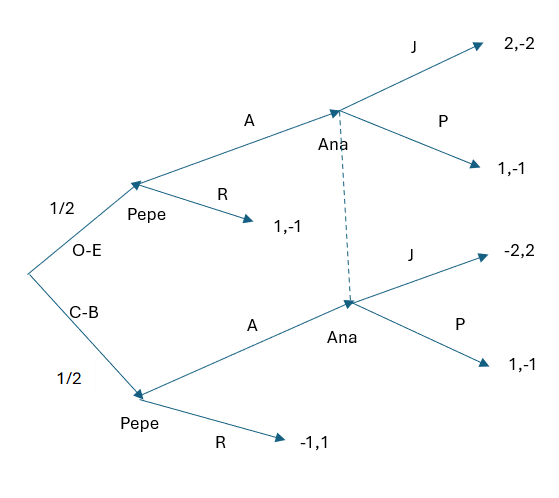
\includegraphics[width=0.8\linewidth]{forma_extensiva} 

}

\caption{\label{forma_extensiva}Diagrama Juego}\label{fig:forma_extensiva}
\end{figure}

La linea discontinua uniendo los dos nodos donde participa la jugadora
Ana denotan que no sabe en que parte del árbol se encuentra, es decir,
hace si apuesta o se retira sin saber de que palo es la carta que saca

Al igual que hicimos en la forma normal de un juego, vamos a
caracterizar la forma extensiva de un juego por los distintos elementos
que intervienen en tal representación

\emph{Definición} Un juego en forma extensiva \(\Gamma\) viene
caracterizado por una 7-tupla:
\[\Gamma=\{J,X,A,\{X_i\}_{i \in J},H,P,U \}\] Los elementos que lo
forman son:

*Conjunto de jugadores que participan en el juego \(J=\{1,\cdots,N\}\).
También es común denotar como jugador 0 a los movimientos que se
realizan aleatoriamente.

*\(X\), conjunto de nodos, que significan una posible situación del
juego. El nodo inicial se representa por \(o\). A partir de este
conjunto podemos diferenciar dos: \(T(X)\) conjunto de nodos terminales
del juego, y \(D(X)=X-T(X)\) los nodos donde algún jugador tiene que
tomar una decisión (no final)

*\(A\), conjunto de todas las posibles acciones del juego

*Para cada jugador \(i \in J\), sea \(X_i\) los nodos en los que el
jugador \(i\) tiene que tomar una decisión

*\(H\), familia de conjuntos de información que son la información que
conoce el jugador en cada nodo.

*Una función de probabilidad \[
\begin{array}{cccc}
P : & H_o \times A & \rightarrow & [0,1] \\
   &  (h,a) & \rightarrow   & P(h,a)
\end{array}
\] que proporciona una probabilidad a las acciones en los que interviene
el azar.

*Función de pagos o utilidad \[
\begin{array}{cccc}
U: & T(X) & \rightarrow & \mathbb{R}^N \\
   &  x & \rightarrow   & U(x)=(U_1(x),\cdots,U_N(x))
\end{array}
\] donde \(U_i(x)\) representa la utilidad que recibe el jugador i.
Podemos suponer que estas funciones son de Von Newmann-Morgenstern

Al igual que hicimos en el apartado anterior, vamos a formalizar el
ejemplo que hemos propuesto en forma extensiva: Tenemos los jugadores
\(J=\{0, Pepe, Ana\} = {0,1,2}\); el conjunto de nodos
\(X=\{0,x_1,x_2,x_3,x_4,x_5,x_6,x_7,x_7,x_8,x_9 \}\); el conjunto de
acciones \(A=\{Ac_1,Ac_2,Ac_3,Ac_4,Ac_5,Ac_6,Ac_7,Ac_8 \}\); los
conjuntos de decisión para cada jugador \(X_i, \ i \in J=\{0,1,2\}\),
\(X_0=\{o \}\), \(X_1=\{x_1,x_2 \}\), \(X_2= \{x_3,x_5 \}\) ; el
conjunto de información de la que disponen los jugadores
\(H=\{ \{o\}, \{x_1\},\{x_2\}, \{x_3,x_5\} \}\); la funcion de
probabilidad para cada una de las acciones en las que interviene el
azar, \(P(\{o\},a)=\frac{1}{2}\) y \(P(\{o\},b)=\frac{1}{2}\); y las
funciones de pagos que reciben los jugadores en los distintos nodos
finales, \(U(x_4)=(1,-1)\), \(U(x_6)=(-1,1)\), \(U(x_7)=(2,-2)\),
\(U(x_8)=(1,-1)\), \(U(x_9)=(-2,2)\), \(U(x_10)=(1,-1)\). Así pues,
vamos a ver el diagrama del juego con esta forma de escribirlo mas
rigurosa:

\begin{Shaded}
\begin{Highlighting}[]
\NormalTok{knitr}\SpecialCharTok{::}\FunctionTok{include\_graphics}\NormalTok{(}\StringTok{"forma\_extensiva\_rigurosa.png"}\NormalTok{)}
\end{Highlighting}
\end{Shaded}

\begin{figure}[H]

{\centering 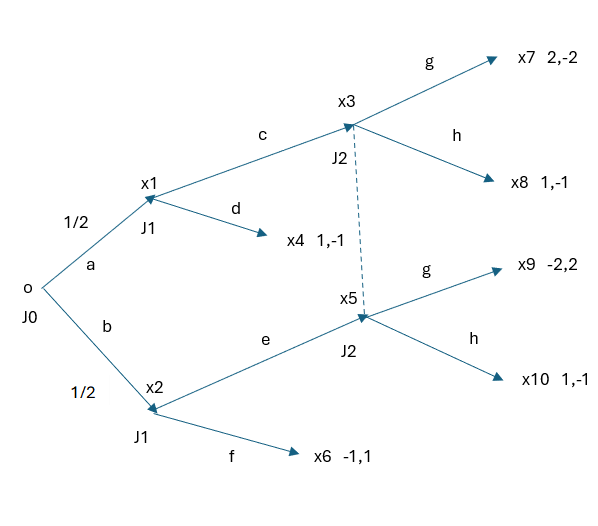
\includegraphics[width=0.8\linewidth]{forma_extensiva_rigurosa} 

}

\caption{\label{forma_extensiva_rigurosa}Diagrama Juego}\label{fig:forma_extensiva_rigurosa}
\end{figure}

\hypertarget{Seccion23}{%
\section{Equilibrio de Nash}\label{Seccion23}}

De manera coloquial diríamos que un juego se encuentra en equilibrio si
ningún jugador obtiene mas utilidad al cambiar su estrategia de manera
unilateral, es decir, cada elección es la mejor respecto al resto de
elecciones de los adversarios, así ningún jugador tiene razones para
cambiar du elección y por tanto el juego se encuentra en equilibrio.
Pasamos a aportar una definición formal de este concepto.

\emph{Definición: Equilibrio de Nash en estrategias puras} Dado un juego
\(G=\{S_1,\cdots,S_n,U_1,\cdots,U_n\}\), un perfil de estrategias puras
\((s_1^*,\cdots,s_{i-1}^*,s_i^*,s_{i+1}^*,\cdots,s_n^*)\) es un
Equilibro de Nash si \[
\forall i \in N, \ U_i(s_1^*,\cdots,s_{i-1}^*,s_i^*,s_{i+1}^*,\cdots,s_n^*) \geq U_i(s_1^*,\cdots,s_{i-1}^*,s_i,s_{i+1}^*,\cdots,s_n^*), \ \forall s_i \ \text{de} \ S_i
\]

A continuación resolveremos los ejemplos que hemos seccionado en las
secciones \(\ref{Seccion221}\) y \(\ref{Seccion222}\)

\hypertarget{Seccion231}{%
\subsection{Resolución de un juego en forma normal}\label{Seccion231}}

Recordamos que tenemos el juego con la siguiente matriz: \[
\begin{array}{c|c|c}
 & \text{Montar} & \text{No Montar} \\
\hline
\text{Montar} & 1,1 & 4,0 \\
\hline
\text{No Montar} & 0,4 & 0,0 \\
\hline
\end{array}
\] En este juego tenemos las siguiente soluciones posibles:
(\(Montar\),\(Montar\)), (\(Montar\),\(No \ Montar\)),
(\(No \ Montar\),\(Montar\)) y (\(No \ Montar\),\(No \ Montar\)).

Comenzamos analizando la solución (\(No \ Montar\),\(No \ Montar\))
suponiendo que es un Equilibrio de Nash. Si la empresa A piensa que la
empresa B no montará el negocio es claro que no le interesa mantener su
decisión en no montar el negocio puesto que su utilidad aumenta de 0 a
4. De esta forma cualquiera de las dos empresas (ocurre lo mismo porque
son simétricas) cambiará su estrategia a montar el negocio.

Ahora analicemos el caso (\(Montar\),\(No \ Montar\)), que tiene un
razonamiento similar al caso (\(No \ Montar\),\(Montar\)), y volvemos a
suponer que es un Equilibrio de Nash. En esta situación, si la empresa B
supiese que la empresa A va a decidir montar el negocio esta cambiara su
estrategia y montaría también el negocio aumentando así su utilidad de 0
a 1. Por lo tanto estas dos opciones (\(Montar\),\(No \ Montar\)) y
(\(No \ Montar\),\(Montar\)) no son un equilibrio de Nash.

De esta forma solo nos quedaría la siguiente solución posible
(\(Montar\),\(Montar\)) que si es un Equilibrio de Nash puesto que ambas
empresas disminuyen la utilidad que perciben si alguna de ellas cambia a
no montar el negocio. De manera gráfica podemos representarlo con la
matriz anterior

\[
\begin{array}{c|c|c}
 & \text{Montar} & \text{No Montar} \\
\hline
\text{Montar} & \underline{1},\underline{1} & \underline{4},0 \\
\hline
\text{No Montar} & 0,\underline{4} & 0,0 \\
\hline
\end{array}
\] y (\(Montar\),\(Montar\)) es el equilibrio de Nash

\hypertarget{Seccion232}{%
\subsection{Resolución de un juego en forma
extensiva}\label{Seccion232}}

Recordemos que hemos llegado al siguiente esquema del juego:

\begin{Shaded}
\begin{Highlighting}[]
\NormalTok{knitr}\SpecialCharTok{::}\FunctionTok{include\_graphics}\NormalTok{(}\StringTok{"forma\_extensiva\_rigurosa.png"}\NormalTok{)}
\end{Highlighting}
\end{Shaded}

\begin{figure}[H]

{\centering 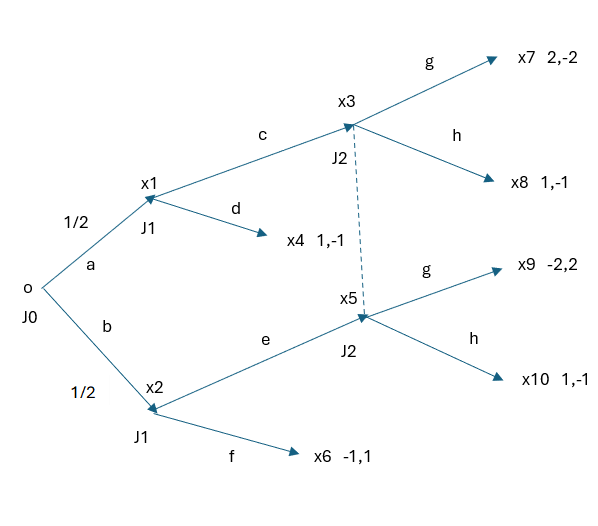
\includegraphics[width=0.8\linewidth]{forma_extensiva_rigurosa} 

}

\caption{\label{forma_extensiva_rigurosa_2}Diagrama Juego}\label{fig:forma_extensiva_rigurosa_2}
\end{figure}

En cuanto al jugador 2, este no sabe en cual de los nodos \(x_3\) o
\(x_5\) se encuentra pues no ve la carta que se saca de la baraja. Así,
se encuentra con una probabilidad de \(\frac{1}{2}\) de estar en \(x_3\)
o en \(x_5\). Si decidimos apostar, el valor esperado a ganar es
\(\frac{1}{2}*(-2) +\frac{1}{2}*2 =0\), mientras que si decide no
apostar y plantarse el valor esperado a ganar es
\(\frac{1}{2}*(-1) +\frac{1}{2}*(-1) =-1\), por lo que el jugador 2
decidirá apostar pues el valor esperado de la utilidad que recibe es
mayor en ese caso.

Por otra parte, el jugador 1 si sabe en cual de los nodos de decisión
\(x_1\) o \(x_2\) pues el si ve la carta que saca del mazo. De esta
forma si se encuentra en el nodo de decisión \(x_1\) puede decidir
plantarse y de esta forma se lleva con probabilidad 1 1 euro, mientras
que si decide apostar, como el jugador 2 siempre decide apostar (g),
tiene un valor esperado de utilidad de
\(\frac{1}{2}*(-2) +\frac{1}{2}*2 =0\) por lo que siempre decidirá
plantarse (d). Si se encuentra en \(x_2\), si decide plantarse (f) tiene
probabilidad 1 de perder 1 euro, mientras que si decide apostar, al
saber igual que antes que el jugador 2 siempre decide g, el valor
esperado de utilidad de \(\frac{1}{2}*2 +\frac{1}{2}*(-2) =0\) que es
mayor así que en este nodo siempre decide e.

\begin{Shaded}
\begin{Highlighting}[]
\NormalTok{knitr}\SpecialCharTok{::}\FunctionTok{include\_graphics}\NormalTok{(}\StringTok{"forma\_extensiva\_equilibrio.png"}\NormalTok{)}
\end{Highlighting}
\end{Shaded}

\begin{figure}[H]

{\centering 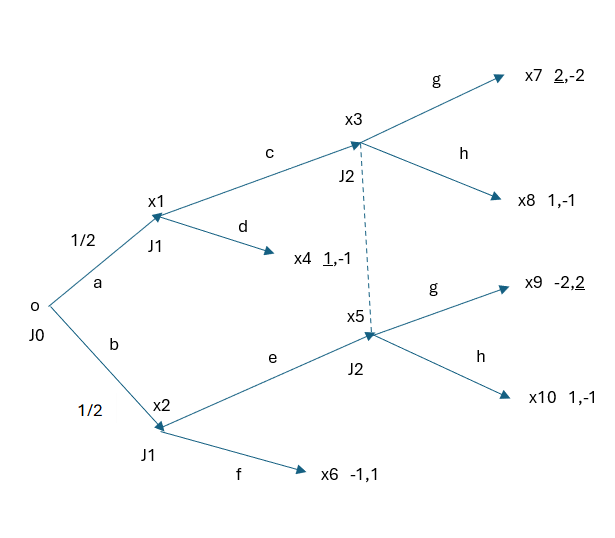
\includegraphics[width=0.8\linewidth]{forma_extensiva_equilibrio} 

}

\caption{\label{forma_extensiva_equilibrio}Diagrama Juego Equilibrio}\label{fig:forma_extensiva_equilibrio}
\end{figure}

\bibliography{bib/library.bib,bib/paquetes.bib}


%


\end{document}
